 \documentclass[../IoMusT.tex]{subfiles}
\begin{document}
\subsection{Prezentarea scurtă a aplicației finale}
Cu ajutorul tehnologiilor software și hardware scopul acestei lucrări a fost de a crea un dispozitiv ce redă sunetele dintr-un instrument muzical în formă de vibrații, venind astfel în ajutor la persoanele cu deficiență de auz. Datorită faptului că celelalte simțuri a acestor persoane sunt mult mai dezvoltate am mers pe ideea de a crea o aplicația care să redea nu numai vibrațiile muzicii ci și să facă și o reprezentare cât mai bună posibilă a acestor note în culori. Astfel utilizatorii vor putea avea și o experiență vizuală plăcută pe lângă cea tactilă și vor putea asocia pentru fiecare vibrație simțită a notă muzicală anume. Pentru a face posibilă acest lucru mai întâi s-a dezvoltat o aplicație pe placa de dezvoltare Raspberry Pi, care are ca scop atât colectarea și trimiterea informațiilor de la pian câtre aplicația Android cât și redarea vibrațiilor cu ajutorul motoarelor LRA. Aplicația Android a venit ca o completare a acestui proiect din nevoia personalizării experienței a utilizatorilor și pentru redarea efectului vizual din datele primite de la placa de dezvoltare Raspberry Pi. În ambele părți s-au folosit tehnologii prezentate în capitolele anterioare iar în cele ce urmează se vor detalia funcționalitățile aplicației și atât metodele de implementare alese cât și cum s-a ajuns la varinata finală în ceea ce privește structura hardware a lucrării.
\subsection{Implementarea aplicației pe placa de dezvoltare RaspberryPi}
\subsubsection{Metode de asamblare aleasă a componentelor hardware}
%adaugare poze cu asamblarea	
Pentru realizarea dispozitivului purtabil s-a folosit nouă bucăți de motoare de tip LRA (a se vedea figura \ref{fig:motors}) conectate da placa de dezvolatre Raspberry Pi.
\begin{figure}[h]
\centering
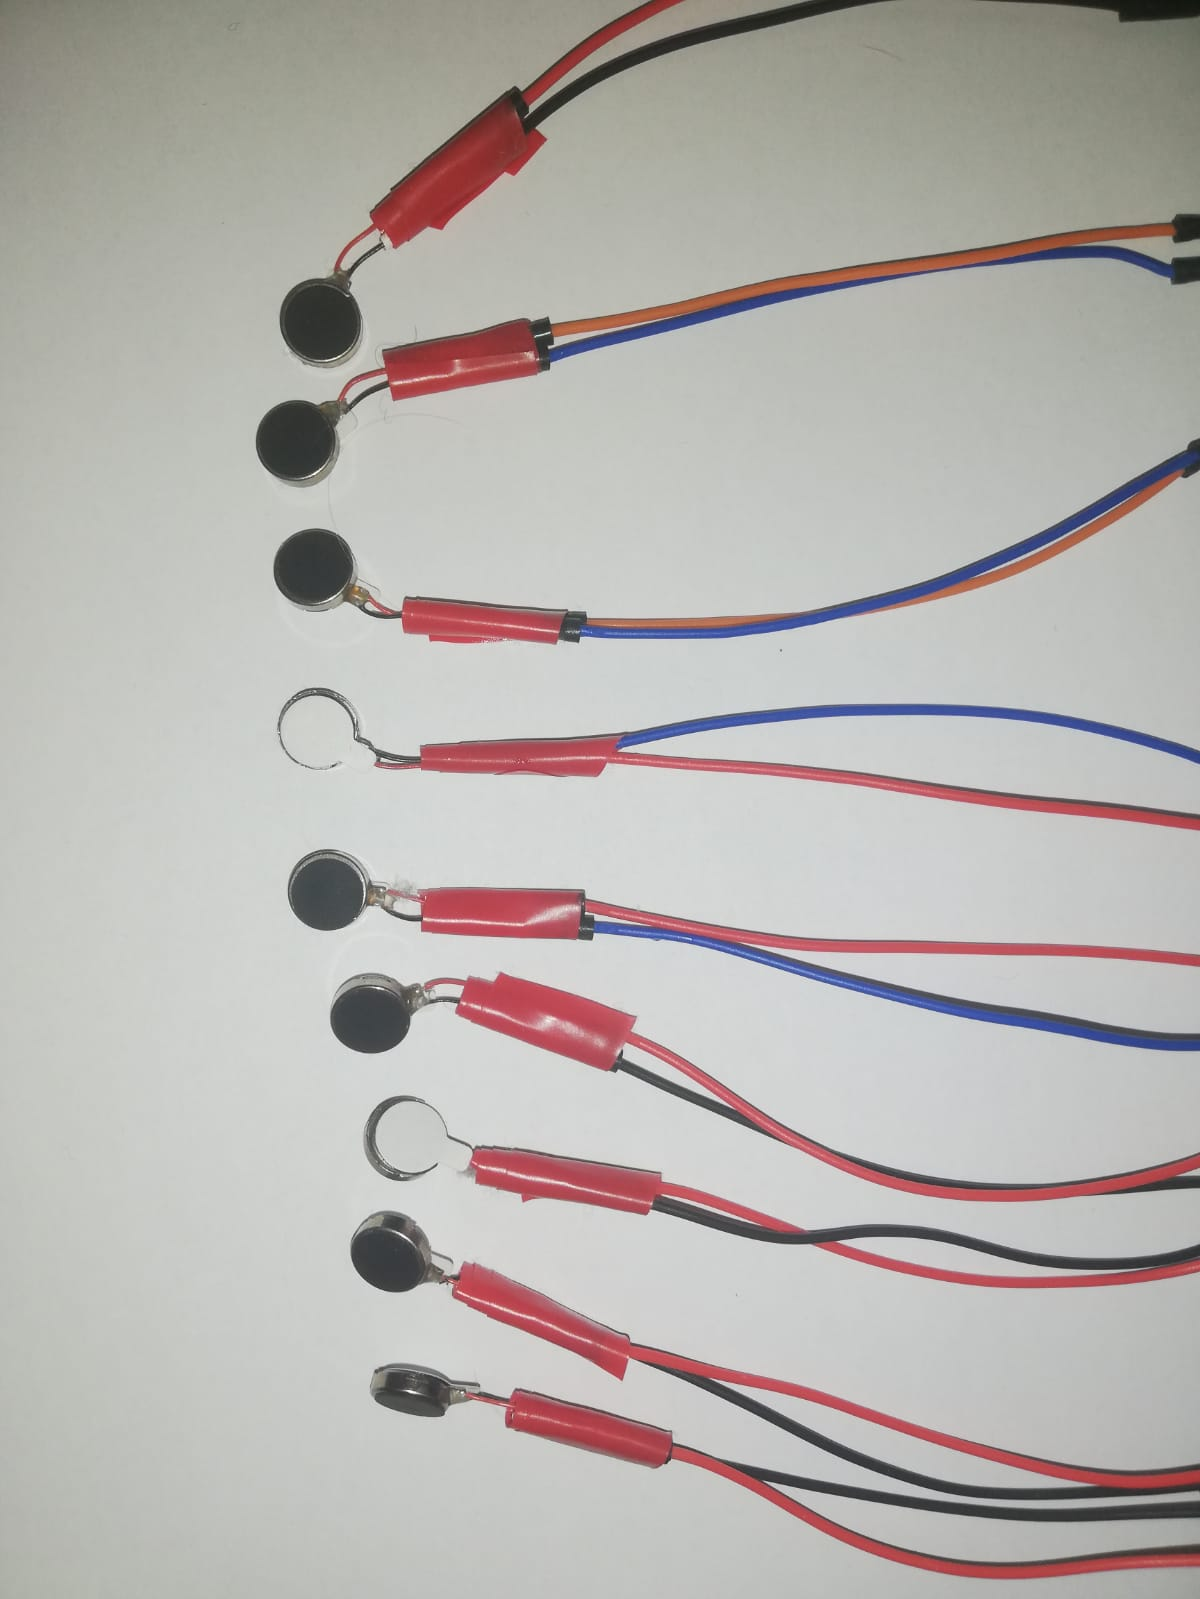
\includegraphics[scale=0.15, angle=270]{motors}
\caption{Motoarele de vibrații}
\label{fig:motors}
\end{figure}  
 Datorită faptului că pentru acest număr de motoare trebuie 9 pini de ground, iar placa are numai 8 la bucăți, s-a folost un breadboard  la care se poate conecta un singur pin de ground. Conectarea s-a făcut cu ajutorul unor cabluri de tip tată-tată și mamă-tată, motoarele de vibrații fiind și ele cositorte de aceste fire pentru un contact mai bun.
\\
\par Numărul total de motoare de vibrații LRA folosite influențează experiența utilizatorului din motive destul de evidente. Mai multe motoare înseamnă vibrații intensificate și de mai multe feluri. Datorită faptului că am folosit un instrument muzical cu o gamă largă de note era evident că pentru a avea un rezultat cât mai bun este nevoie ca vibrațiile resimțite să provină din mai multe astfel de dispozitive. Nu s-au folosit un număr mai mare decât nouă din cauza posibilităților de echipamente hardware. Modul în care acestea sunt distributie și vibrează este în felul următor: folosind un pian electric cu 61 de clape am împărțit aceste clape în trei categorii de note muzicale. Primele două octave (adică notele joase) reprezintă prima categorie. A doua categorie reprezintă notele din mijloc, aceasta fiind formată numai dintr-o ocatvă. Ultima categorie este reprezentată de cele două octave rămase adică notele cele mai înalte. Fiecărui astfel de categorie i se atribuie trei motoare. Când se va apăsa o clapă una dintre cele trei categorii de motoare vor începe să vibreze la o anumită valoare și frecvență calculată. Metoda prin care au fost calculate aceste categorii se poate observa în figura \ref{fig:range} unde se verifică numărul MIDI a notei muzicale iar în funcție de asta se va returna un boolean.
\begin{figure}[h]
\centering
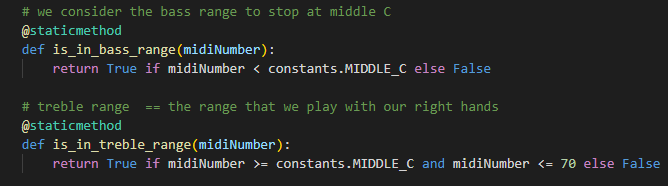
\includegraphics[scale=0.75]{range}
\caption{Împărțirea motoarelor în categorii}
\label{fig:range}
\end{figure}  
\\
\par Breadbourd-ul folosit pentru prototipare este unul cu 830 de puncte, având destul loc pentru conectarea motoarelor. Pentru conecatrea la ground s-a folosit un singur pin de pe placa de dezvoltare  Raspberry Pi, acesta fiind conectat la rândul corespunzător de pe breabdoard. Cei nouă pini folosiți pentru alimentarea cu tensiune sunt: 14, 15 și 18 pentru prima categorie, 17, 27, 22 pentru a doua respectiv 10, 9 și 11 pentru ultima categorie de motoare, fiecare dintre aceștia putând fi programat pentru modularea lățimii pulsului. Modul în care firele și motoarele de vibrații au fost conectate la breadboard se poate vedea în diagrama fritzing din figura \ref{fig:breadboardConnection}. În total sunt zece fire conectate, unul pentru ground iar restul pentru pinii menționați mai sus.
\begin{figure}[h]
\centering
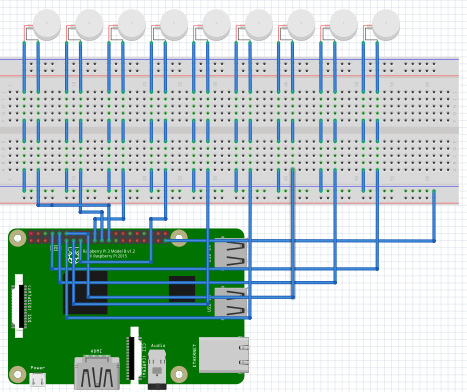
\includegraphics[scale=0.8]{fritzing}
\caption{Diagramă fritzing}
\label{fig:breadboardConnection}
\end{figure}  
\newpage
\subsubsection{Folosirea echipamentului hardwer de către utilizatori}
Dispozitivul este destinat persoanelor  cu dizabilități. Folosirea acestuia este ușor, utilizatorul trebuind doar să pună palma (să facă contact) pe motoarele de vibrații. În momentul în care se pornește placa de dezvoltare Raspberry Pi conectată la pian și o persoană cântă la instrumentul respectiv, utiliztorul poate deja să simtă vibrațiile. Latența dintre momentul în care o clapă a fos apăsată și momentul în care motoarele încep să vibreze va fi una de 0.02 secunde. Totodată dacă o clapă a fost ținută apăsată mai mult timp, asta însemnând că se crează un sunet mai lung, motoarele nu vor vibra pe toată durata acestui timp, utilizatorul simțind vibrațiile numai 0.02 de secunde. Cu toate că acest timp pare puțin, datorită faptului că sunt mai mult motoare acesta este îndeajuns și chiar favorizează mai ales în cazul în care ritmul muzicii este una foarte rapidă. Dacă aplicația este conectată la o sursă de alimentație, ea rămâne pornită până când se întrerupe curentul. Aplicația rulează și în momentul în care pianul nu este încă pornit (fiind vorba despre un pian electric). Utilizatorul va putea opri vibrațiile numai din aplicația mobilă ce va fi prezentată în subcapitolele ce urmează.
\subsubsection{Metoda de calculare folosită pentru motoarele de vibrații}
Calcularea intensității și a frecvenței cu care vibrează un motor se face pe baza notei MIDI primite de la pian. Nota muzicală cântată ajunge sub forma unui număr în programul nostru asta însemnând că cu cât e mai mare numărul respectiv cu atât nota muzicală cântată este mai înaltă. Pentru calcularea frecvenței, dintr-o notă muzicală, cu care vibrează un motor există formulă și s-a discutat despre asta în capitolul anterior. Datorită faptului că aceste schimbări de frecvențe pot fi simțite foarte puțin la o valoare de vibrație constantă, este necesar și calcularea acestor valori.
\\
\par Știm că un motor de vibrații în cazul nostru poate lua valori între 0 și 1, asta însemnând că cu valoarea 0.5 motorul ar avea o vibrație decentă, fără prea multă putere. Luând această valoarea ca baza, am folosit regula de trei simpli pentru a calcula valoarea notei cântate. Nota care va vibra cu valoarea 0.5 am ales să fie A4 (la) fiind referința de ton care sunt reglate celelalte instrumente muzicale, acesta având și o frecvență întreagă (440 Hz) și fiind și clapa care este aprope de mijlocul pianului. O parte a metodei în care se calculează aceste valori se poate vedea în figura \ref{fig:calculateValue}.
\begin{figure}[h]
\centering
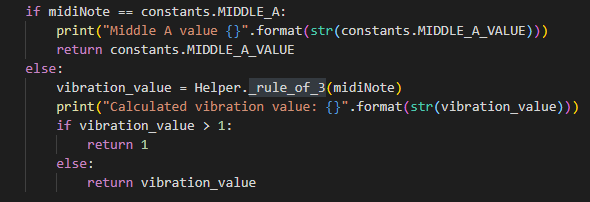
\includegraphics[scale=0.9]{calculateValue}
\caption{Calcularea valorii unei vibrații}
\label{fig:calculateValue}
\end{figure}  
 Știind că nota la este baza după care se calculează celelate note, apăsarea acestuia nu va apela metoda ce returnează rezultatele de la regula de 3 simpli. În cazul în care valoarea calculată este mai mare decât 1, se va returna valoarea 1 datorită faptului că biblioteca PWMOutputDevice va arunca excepție în caz contrar. Pentru valori mai mici de 0 nu o să avem caz pentru că este imposibil să primim un număr negativ. Metoda care calculează regula de trei simpli este prezentată în figura \ref{fig:ruleOf3}, unde \verb|MIDDLE_A| reprezintă numărul MIDI a notei muzicale A4 iar (69) iar \verb|MIDDLE_A_VALUE| este valoarea 0.5. Cu această metodă vom avea o distribuire uniformă în ceea ce privește valorile pentru fiecare notă. Notele joase vor fi simțite cu o intensitate mai mare în timp ce notele mai înalte se vor simți mai puțin (în acest caz valoarea nu scade prea mult, va fi în jurul valorii 0.2, ceea ce încă se poate simți). În cazul nostru cea mai mare valoare va fi în jur de 0.8, acesta ajungând la 1 doar în cazul în care conectarea se face la un pian cu mai multe octave sau dacă utilizatorul va intensifica aceste valori din aplicația de pe telefon.
\begin{figure}[h]
\centering
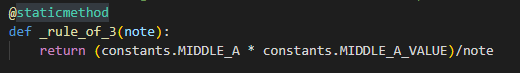
\includegraphics{ruleOf3}
\caption{Regula de 3 simpli}
\label{fig:ruleOf3}
\end{figure}  
\\
\par Formula cu care se calculează frecvența notelor muzicale a fost deja descris în subcapitolul 3.3. Utilizarea acestor valori (înafară de setarea vibrației) se va discuta în subcapitolul ce urmează, acesta fiind folosit și în aplicația Android.
\\
\par Toate valorile calculate au fost afișate în consolă pentru a putea urmării corectitudinea algoritmilor și valorilor calculate. Un exemplu, unde s-a apăsat clapa sol diez din octava din mijloc, se poate observa în figura \ref{fig:gSharp}, unde pe lângă aceste valori calculate, se afișează atât nota apăsată cât și categoria de motoare în care aparține. Pentru calcularea intensității cu care vibrează aceste motoare, se poate lua în considerare și forța cu care clapa respectivă a fost apăsată. O apăsare mai puternică înseamnă un sunet mai tare, mai puternic. Pentru că pianul folosit în dezvolatrea acestui proiect este unul vechi, iar aceste valori nu sunt trimise corecte, am decis să nu iau în considerare acest factor. După cum se observă și din figură, această velocitate este 0, ceea ce e incorect, având în vedere că valoarea implicită trebuie să fie aproximativ 65 \cite{Mido}.
\begin{figure}[h]
\centering
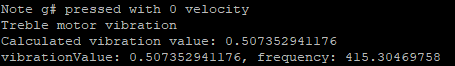
\includegraphics{gSharp}
\caption{Valori calculate în consolă}
\label{fig:gSharp}
\end{figure}  
\subsubsection{Comunicarea dintre firele de execuție} 
Datorită faptului că această aplicație se rulează pe mai multe fire de execuție este important să avem o comunicare bine sincronizată dintre aceastea în momentul cănd dorim să schimbăm mesaje între ei. Utilizarea socket-urilor impune folosirea unui fire de execuție separat ceea ce înseamnă că în momentul trimiterii sau a primii unor date, trebuie să avem acces la o memorie comună la care au acces ambele fire de execuție pentru a putea face schimb de informații. În cazul acestei aplicații trimiterea acestor datelor se face de pe ambele părți: atât aplicația Android cât și cea de pe placa de dezvoltare trebuie să trimită și să primească informații, ce vor fi parsate în următoarele etape.
\\
\par Gestionarea memoriei comune în aplicația de pe placa de dezvoltare se întâmplă cu ajutorul unei cozi. În momentul în care se primesc date, acestea sun decodate și puse în coadă. Celălalt fir de execuție, care trebuie să parseze aceste mesaje, preia informațiile din ea. Coada nu râmăne niciodată plină, mereu se scoate toată informația din ea de către celălalt fir de execuție. Pentru a putea implementa aceste acțiuni avem nevoie să știm momentul în care putem prelua aceste informații din coadă, din moment ce acestea nu vin încontinuu.
\\
\par Evenimentele din biblioteca \verb|threading| ne vin în ajutor în momentul în care dorim să primim o notificare că s-a întâmplat un lucru, fiind cel mai simplu mod de a comunica unui al fir de execuție că a avur loc a acțiune. Acestea funcționează ca niște booleane care pot fi setate în momentul în care s-a întâmplat o acțiune. În cazul nostru de fiecare date cănd se pune sau se ia un element în coadă,
\begin{figure}[h]
\centering
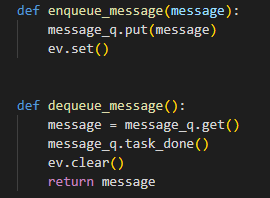
\includegraphics[]{ev}
\caption{Setare eveniment}
\label{fig:ev}
\end{figure}  
 acest eveniment este setat pe \verb|True| respectiv pe \verb|False|  (a se vedea figura \ref{fig:ev}).
 Verificarea stării acestui eveniment se face prin apelarea metodei \verb|is_set()|.
Setarea evenimentului se verficiă în momemntul în care citim datele de la pian. Datorită faptului că mesajele ce vin de pe aplicația Android influențează modul în care motoarele vor vibra, trebuie să preluăm și să parsăm aceste mesaje înaintea să setâm valoarea și frecvența motoarelor. În momentul în care acest eveniment a fost setat pe \verb|True|, se apelează o metoda din figura \ref{fig:processEv} care va procesa aceste date iar în funție de rezultate se vor modifica niște valori dintr-un dicționar. Aplicația a fost dezvoltată în așa fel încât mesajele primite să fie compuse mereu din două cuvinte, ușurând astfel parsarea acestora. După ce mesajul a fost scos din coadă, evenimentul va fi setat pe \verb|False| până când un nou mesaj va fi introdus.
\begin{figure}[h]
\centering
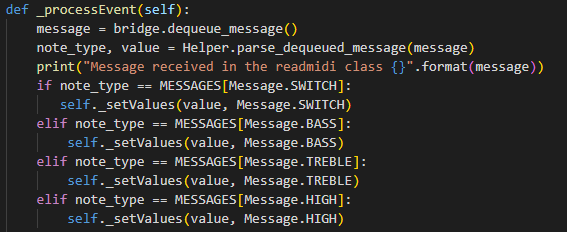
\includegraphics[scale=0.7]{processEv}
\caption{Parsare mesaje}
\label{fig:processEv}
\end{figure} 
\\
\par Soluția asta ne oferă o reacție rapidă în ceea ce privește controlarea dispozitivului cu o aplicație mobilă. În momentul în care utilizatorul dorește să regleze sau să oprescă vibrațiile, timpul de răspuns de către aplicația de pe placa de dezvoltare va fi una rapidă. 
\subsection{Integrarea unei aplicații mobile în proiect}
\subsubsection{Nevoia de folosire a unui aplicații Android}
Aplicația de placa de dezvoltare Raspberry Pi, după cum s-a discutat și în capitolele anterioare, oferă posibilitatea redării muzicii cântate la pian în formă de vibrații. Utilizatorul acestui dispozitiv, fără o aplicație conectată, nu are nici un fel de control asupra acestor lucruri, nu poate să intervină să oprescă sau să personalizeze vibrațiile simțite. Crearea unei aplicații Android pentru acest dispozitiv nu are scopul doar de a controla aceste vibrații dar și de a oferi un feedback vizual în ceea ce privește aceste note muzicale. 
\\
\par În subcapitolele ce urmează vor fi prezentate atât funcționalitățile incluse în aplicația Android cât și algoritmii aleși pentru implementarea acestora.
\subsubsection{Folosirea interfeței aplicației mobile}
%\begin{wrapfigure}{r}{0.5\textwidth}
%\begin{center}
%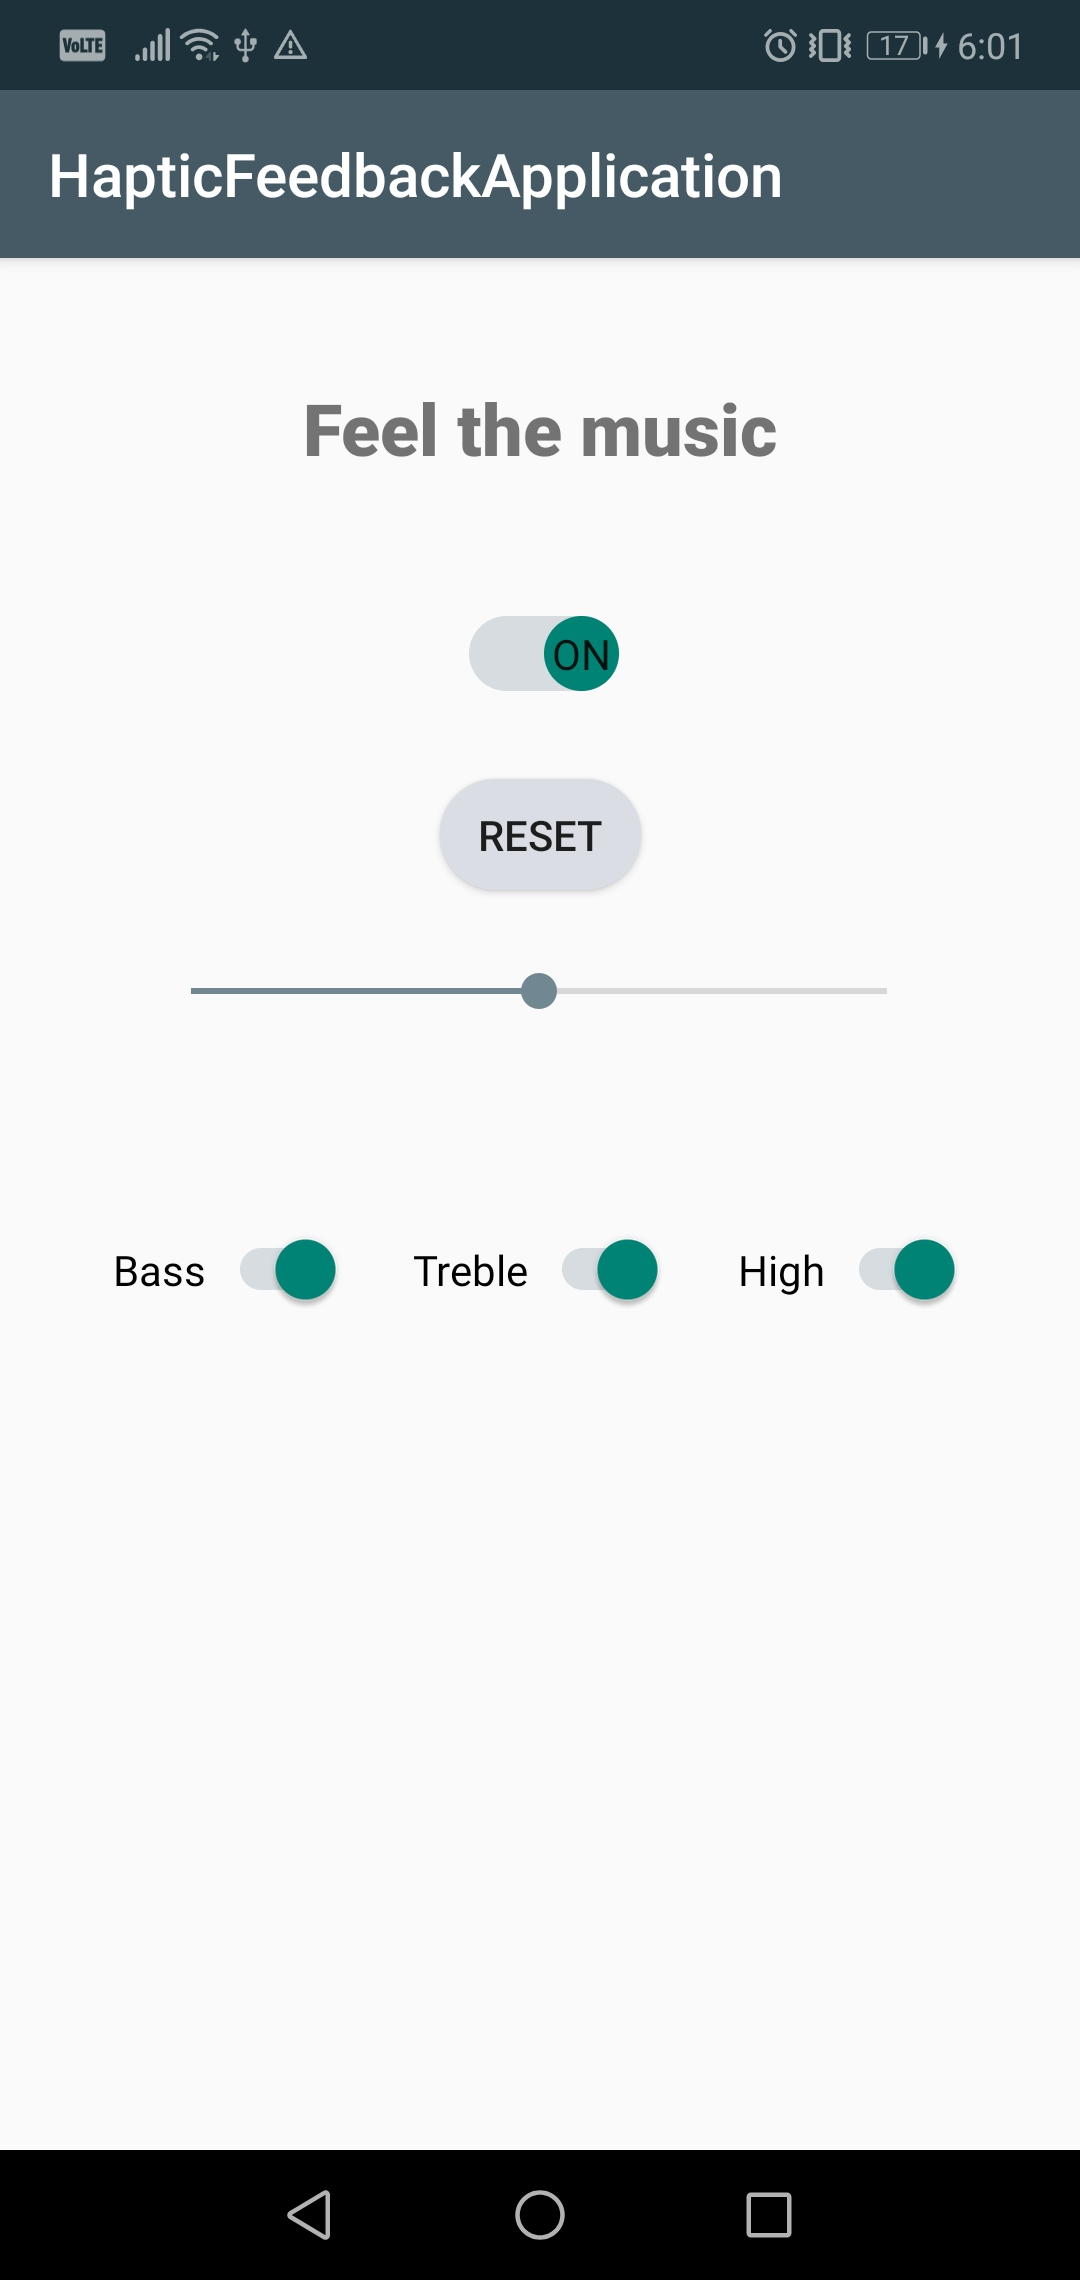
\includegraphics[scale=0.11]{application}
%\caption{Interfață aplicație mobilă}
%\label{fig:application}
%\end{center}
%\end{wrapfigure}
Aplicația Android dezvoltată este una cu o singură activitate cu mai multe funcționalități ce permit utilizatorilor manipularea motoarelor de vibrații.
 Pe lângă acest control, aplicația dispune și de o reprezentare prin culori a notelor muzicale, valorile RGB fiind calculate cu ajutorul frecvențelor primite de pe placa de dezvoltare RaspberryPi. Modul prin care se conectează aplicația la placă este prin intermediul unei adrese IP statice, utilizatorul neavând nevoie de o autentificare. Dacă conectarea s-a făcut cu succes, va apărea un popup cu mesajul respectiv și titlul aplicației își va schimba culoare din gri în verde. Se poate observa interfața aplicației mobile în figura \ref{fig:application}. În continuare se vor prezenta și se vor descrie funcționalitățile aplicației mobile.
\begin{figure}[h]
\begin{center}
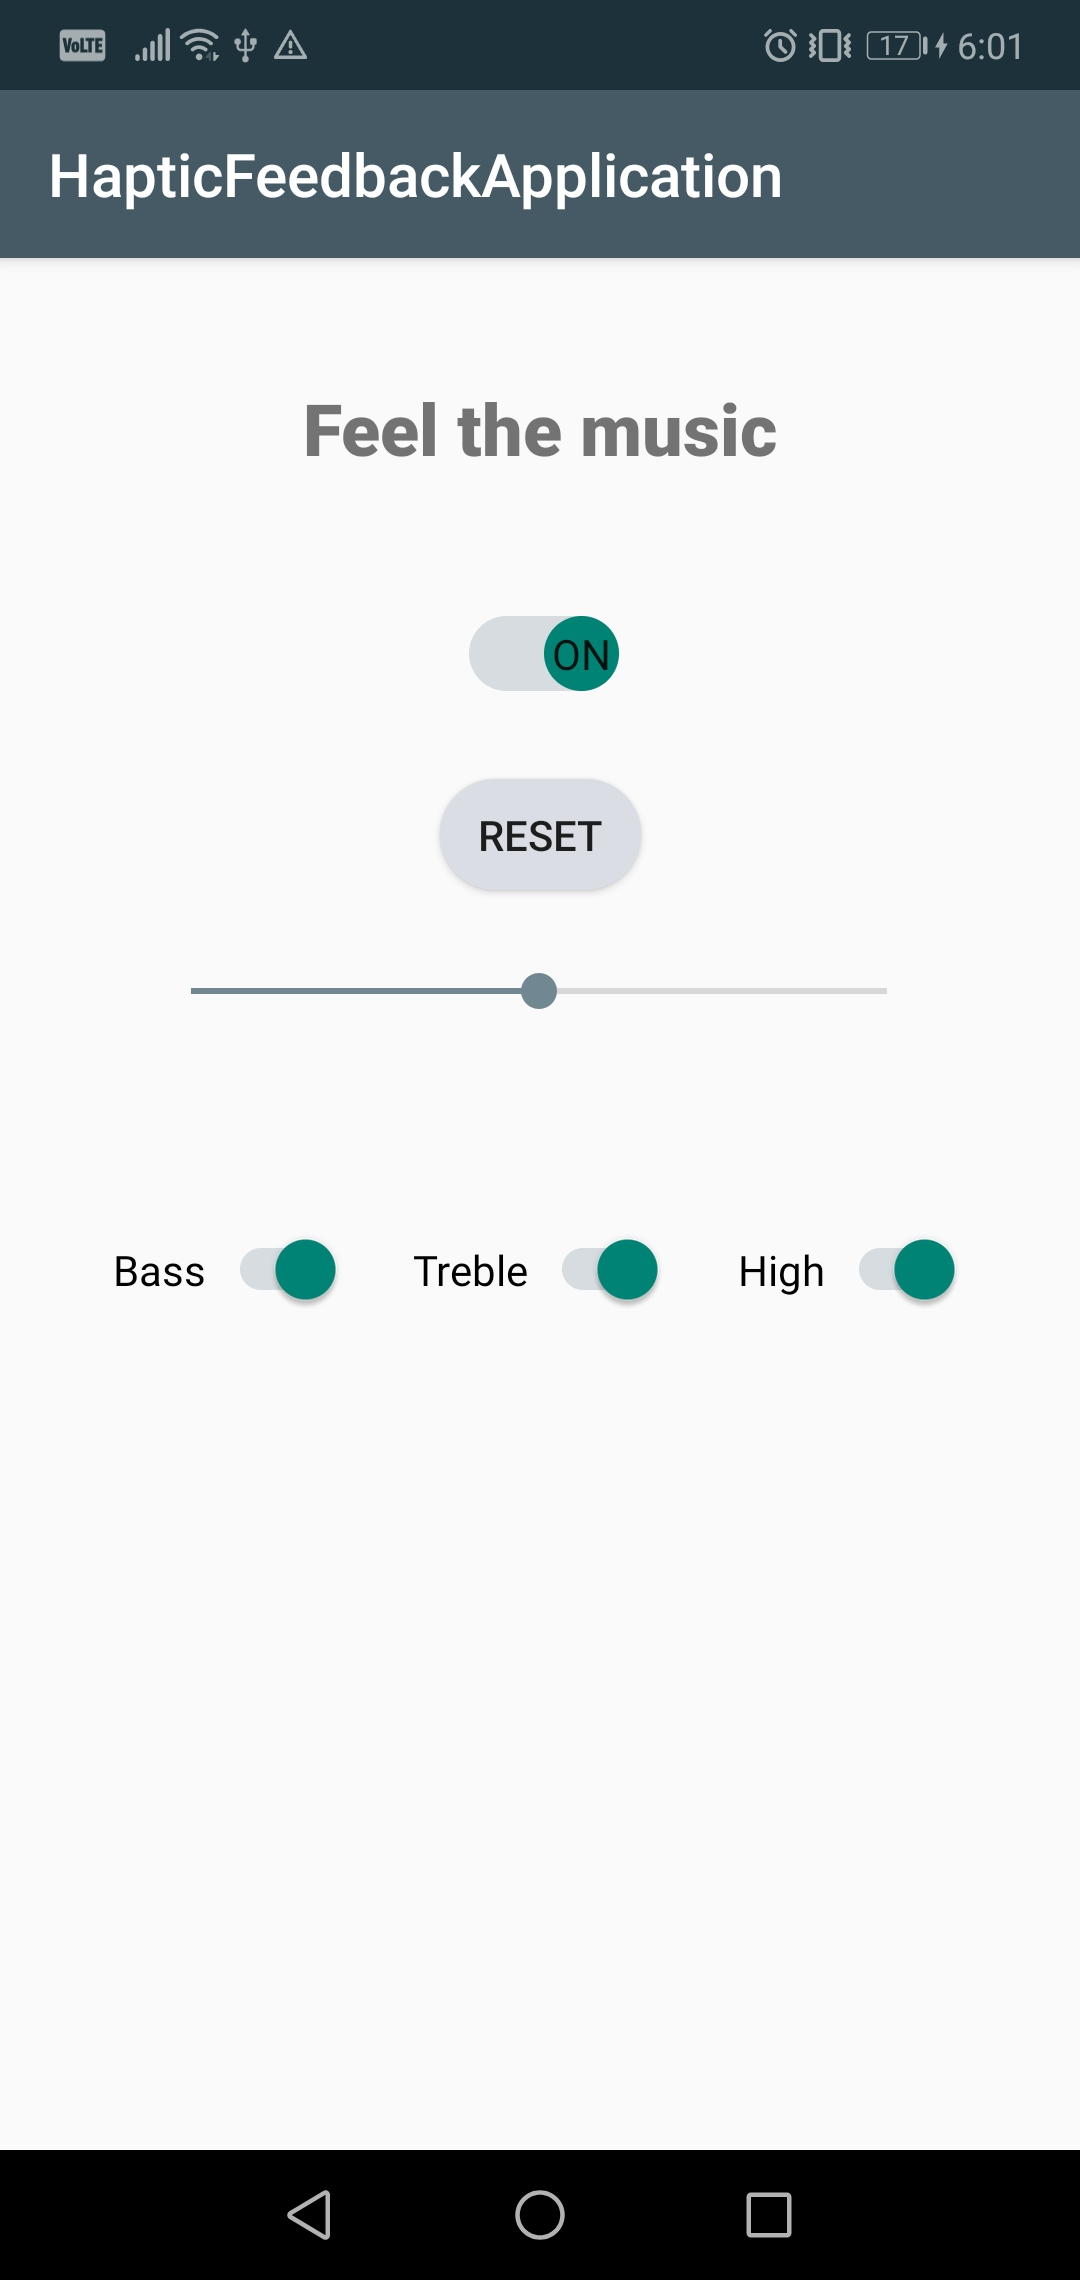
\includegraphics[scale=0.11]{application}
\caption{Interfață aplicație mobilă}
\label{fig:application}
\end{center}
\end{figure}
\\
\par Aplicația dispunde de mai multe butoane de comutare printre care se află și buton de oprire și pornire. La deschiderea aplicației acest buton este setat în mod implicit de pornit. Dacă utilizatorul va trage butonul de comutare spre stânga, se vor opri toate vibrațiile.
\\ %reformulare
\par Utilizatorul are posibiliatea să controleze toate cele trei categorii de motoare, atașate de placa de dezvoltare, prin butoane de comutare. Aceste motoare pt fi oprite sau repornite fiecare în parte, separat. Ca și la butonul de oprire și pornire, și la aceste butoane este setat în mod implicit la pornirea aplicației să fie pe opțunea de pornit. Nevoia acestor butoane se poate explica prin faptul că persoanele surde de cele mai multe ori simt numai basul muzicii prin intermediul difuzoarelor. Pentru că aplicația dezvoltată redă și virbațiile și notelor foarte înalte, am considerat implementarea acestui funcționalități una de folos. 
\\
\par Cu ajutorul unei bare de progrese se poate seta intensitatea cu care se pot simți vibrațiile. Bara poate lua valori întregi de la 0 până la 100, valoarea implicită fiind cel de 50, la care vibrațiile au exact valorile calculate în aplicație. Schimbarea cursorului va afecta vibrațiile cu
 până la 0.2 de valori. Funcționalitatea acestui component se poate cel mai ușor compara cu cel al schimbării volumului. De fiecare dată când se va schimba bara de progres, va apărea pe partea de jos a ecranului un mesaj popup cu valoarea curentă a barei de progres, care va dispărea după o perioadă scurtă de timp. Cu ridicarea intensității până la valoarea maximă utiizatorul va putea simți notele joase cu valoarea de vibrație maximă admisă de motoare.
\\
\par Există și posibilitatea resetării tuturor acestor componente la valoarea implicită cu ajutorul butonului reset. Singurul lucru pe care nu îl resetează este butonull de oprire/pornire, care își va păstra starea în care se află la momentul respectiv.
\\
\par Pe partea de jos a ecranului se află un ImageView, inițial de culoare albă, care are ca scop redarea prin culori a notelor muzicale. De fiecare dată când s-a apăsat o clapă pe pian și s-a trimis valoarea frecvenței notei respective, utilizatorul va vedea o schimbare de culoare pe baza notei respective. Modul în care aratâ ecranul când s-a produs o apăsare de notă pe pian se poate observa în figura \ref{fig:applicationPressed}.
\begin{figure}[h]
\begin{center}
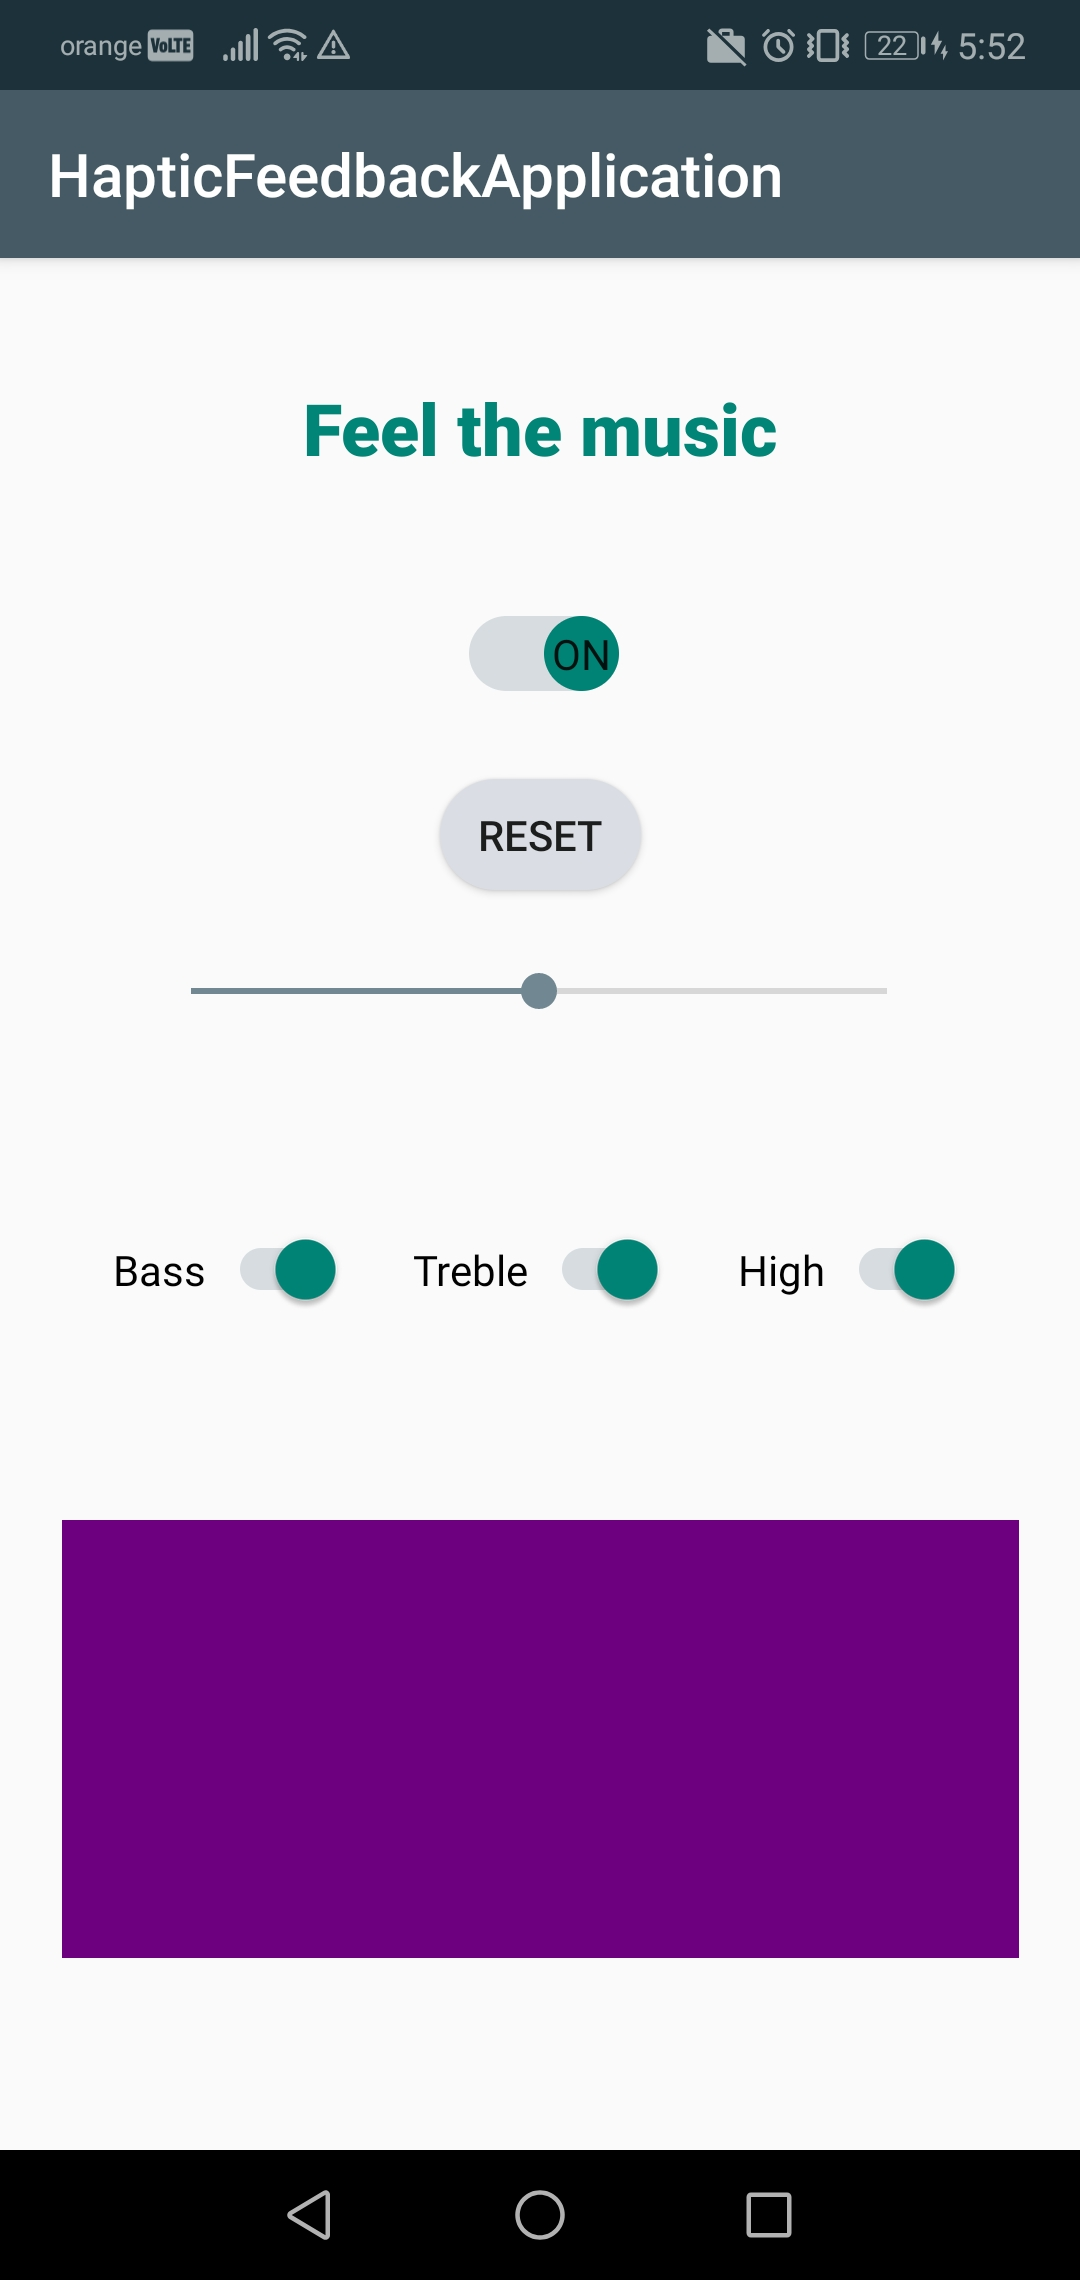
\includegraphics[scale=0.11]{applicationPressed}
\caption{Interfață aplicație mobilă}
\label{fig:applicationPressed}
\end{center}
\end{figure}
\\
\par Pe durata timpului de folosire a aplicației utilizatorul poate să-și blocheze telefonul fără să piardă modificările. Conexiunea cu placa de dezvoltare Raspberry Pi se va pierde doar în momentul în care se iese total din aplicație. Atunci se pierd toate setările făcute, iar valorile de la motoarele de vibrații o să se reseteze la cele implicite.
\\
\par Instalarea aplicației este una foarte ușoară și se întâmplă cu ajutorul unui fișier cu extensia apk. Pe durata instalării, aplicația nu va cere nici o fel de permisiune.
\subsubsection{Metoda de calcul pentru modificarea intensităților motoarelor de vibrații}
Modificarea intensităților cu care motoarele conectate vibrează este o funcționalitatea a cărui implementare necesită recalcularea valorilor cu ajutorul niștor formule. Am încercat să aleg metoda cea ma corectă de a calcula aceste schimbări astfel încât rezultatul final să fie unul cât mai corect și mai vizibil. Pe partea de aplicație Android am implementat numai partea de interfață a acestei funcționalități, urmând ca în aplicația de pe placa de dezvoltare Raspberry Pi să se facă calculelel necesare.
\\ %limita
\par În aplicația Android schimbarea valorilor a fost implementată cu ajutorul unei bare de progres. Aceste bare, a căror progrese pot fi setat manual de către utilizator, pot lua valori întregi într-o anumită limită ce poate fi specificată în cod. În cazul nostru aceste valori sunt cuprinse între 0 și 100, valoarea implicită fiind 50 datorită faptului că intensitatea poate să și scadă, nu numai să crească. Astfel dacă un utilizator trage bara de progres până la valoarea 0, intensitatea va scădea iar la 100 va crește cu până la 0.2 de valori. În momentul în care aplicația a sesizat o schimbare de valori în bara de progres, se trimite valoarea curentâ prin socket câtre aplicația de pe placa de dezvoltare. Mesajul se trimite sub forma unor două cuvinte (a se vedea figura \ref{fig:sendProgress}), toate mesajele fiind trimise așa pentru o parsare mai ușoară și corectă. Astfel în aplicația scrisă în python, prin despărțirea acestor două cuvinte, putem să ne dăm seama ușor operațiile ce trebuie făcute după primirea mesajelor.
\begin{figure}[h]
\centering
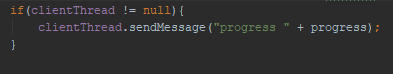
\includegraphics[]{sendProgress}
\caption{Trimiterea valorii barei de progres}
\label{fig:sendProgress}
\end{figure} 
\\
\par Calculul pentru schimbarea valorii a fost gândită în felul următor: dacă utilizatorul schimbă bara de progress cu 10 valori (de la 50 la 60 sau de la 50 la 40), intensitatea motoarelor se va ridica sau va scădea cu același procent. Așadar pentru o schimbare de 50 de valori (de la 50 la 100 sau de la 50 la 0) va produce în ambele cazuri o recalculare a valorilor de vibrații de 0.2. În aplicația python, cu ajutorul unui dicționar este păstrat valoarea implicită a acestui porgres (50), astfel modificările de valori se vor întâmpla doar în cazul în care acest progres este diferit de valoarea implicită (a se vedea figura \ref{fig:not50}). În această situație este calculat o valoarea adițională care va fi adăugat la valoarea calculată în mod normal.
\begin{figure}[h]
\centering
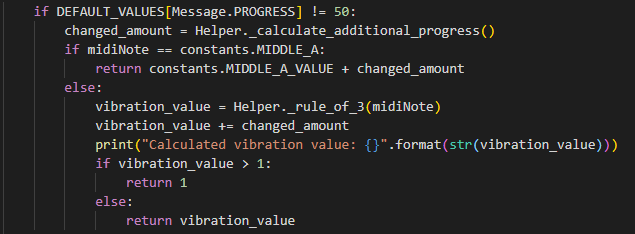
\includegraphics[scale=0.75]{progressNot50}
\caption{Calculul valorii cu pogres schimbat}
\label{fig:not50}
\end{figure} 
\\
\par Metoda care calculează valarea adițională care va fi adăugată are la bază o regulă de trei simpli. Se verifică dacă valoarea progresului trimis de pe aplicația Android este mai mic sau mai mare decât 50 pentru a ști dacă noua valoarea returnată trebuie sau nu să fie un număr negativ. Pentru că știm că valoarea maximă cu care se poate schimba bara de progres este de 50 și în cazul acesta intensitatea se schimbă cu 0.2, este ușor de calculat cu cât se schimbă intensitatea motoarelor de vibrații dacă valoarea acestui bare este diferit de 50.
Acest calcul se poate observa în figura \ref{fig:additionalProgress}, unde \verb|MAX_MIN_PROGRESS_VALUE| este valoarea cu cares se poate schimba intensitatea motoarelor de vibrații iar \verb|DEFAULT_VALUE_FOR_SLIDER| este valoarea implicită pe care o are bara și totodată valoarea maximă cu care se poate schimba cea implicită.
\begin{figure}[h]
\centering
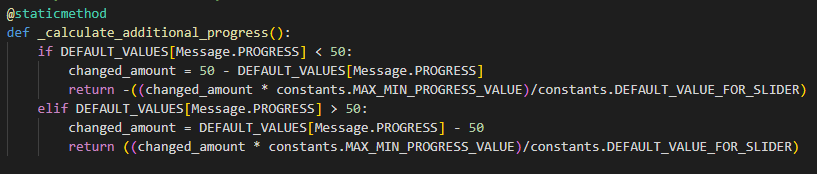
\includegraphics[scale=0.6]{additionalProgress}
\caption{Progress adițional}
\label{fig:additionalProgress}
\end{figure} 
\\
\par Exemplificarea acestui funcționalități se poate observa în figura \ref{fig:beforeAfter} , unde prima parte a imaginii reprezintă nota muzicală fără schimbarea intensității iar partea a doua cu o schimbare de intensitate cu 0.2 valori.
\begin{figure}[h]
\centering
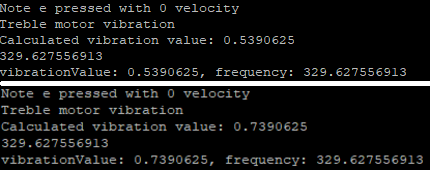
\includegraphics[scale=0.8]{beforeAfter}
\caption{Exemplu schimbare intensitate}
\label{fig:beforeAfter}
\end{figure} 
\subsubsection{Realizarea comunicari și trimiterii mesajelor cu aplicația RaspberryPi}
Metoda aleasă pentru comunicarea între placa de dezvoltare Raspberry Pi și aplicația Android este cea cu socket-uri, aceasta fiind cea mai potrivită nevoilor noastre. Partea de server a acestei comunicări a fost implementată pe placa de dezvoltare datorită faptului că dorim ca serverul să ruleze încontinuu și să poate accepta conexiunea clienților, în cazul nostru aplicației mobile. Odată cu pornirea aplicației python, serverul pornește și el ascultând conexiuni de la clienți cu adresa și portul sepcificat. Prin metoda în care a fost implementată socket-ul server pe aplicația Raspberry Pi, se pot conecta mai multe apicații mobile la același dispoziti.
\\
\par Forma prin care se trimit mesajele de la client la server sau invers ușurează parsarea acestora mai ales dacă mesajele respective sunt compuse din main multe cuvinte. În cazul aplicației mobile, toate mesajele trimise câtre server sunt formate din două cuvinte, primul cuvânt reprezentând componenta pentru care se întâmplă acțiunea iar al doilea fiind acțiunea în sine (de exemplu oprit, pornit). Dacă utilizatorul dorește să oprească vibrațiile de la notele joase, mesajul care va fi trimis prin socket este "bass off". 
\\
\par Datorită faptului că se face o reprezentare prin culori a notelor muzicale cu ajutorul frecvențelor, de fiecare dată când se apasă pe o notă muzicală și se calculează frecvența, serverul trebuie să trimită acest mesaj aplicației mobile. Calcularea valorilor RBG se face pe partea de client pentru că trimiterea a trei valori într-un mesaj este mai complicat când vine vorba despre parsarea acestora. Fiecare frecvență calculată, dacă o transformăm în șir de caractere, are o lungime de 13 caractere astfel știm că în momentul primirii mesajului pe aplicația mobilă trebuie să avem acest număr de caratere. Pentru că mesajul vine codat, primirea acestuia se face cu ajutorul unui vector de octeți care vor trasnformate în șir de caractere și apoi într-un număr real în virgulă mobilă (a se vedea figura \ref{fig:freqParse}).
\begin{figure}[h]
\centering
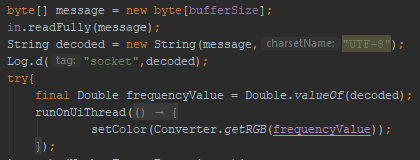
\includegraphics[]{freqParse}
\caption{}
\label{fig:freqParse}
\end{figure} 
\subsubsection{Integrarea vizualizării culorilor cu ajutorul frecvențelor}
Pentru o reprezentare vizuală a notelor muzicale cu ajutorul culorilor există mai multe abordări datorită faptului că este greu de găsit o mapare exactă, unu-la-unu, între note muzicale și culori. În această situație sinestezia poate juca un rol important în găsirea acestei corespondențe însă din păcate nici această abordare nu este una exactă din cauza faptului că fiecare persoană în parte poate percepe altfel simțurile, având o imagine diferită despre tot ce înseamnă conconrdanța dintre sunet și culoare. Cea mai cunoscută astfel de asociere este a lui Scriabin care a creat un cerc a notelor muzicale folosind intervale de cvarte și cvinte perfecte așa cum se poate vedea și în figura \ref{fig:scriabin} \cite{scriabin}. Datorită faptului că această reprezentare poate fi una neexactă și bazată numai pe niște simțuri ce pot varia de la o persoană la alta, am decis să abordez acest subiect într-un mod mai științific, făcând o mapare cât se poate de realistă folosind frecvențele notelor muzicale. 
\begin{figure}[h]
\centering
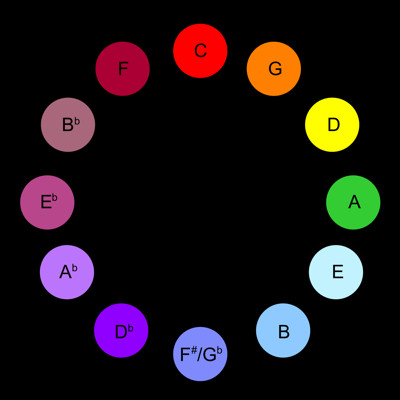
\includegraphics[scale=0.4]{scriabin}
\caption{Sinestezia}
\label{fig:scriabin}
\end{figure} 
\\
\par Spectrul electromagnetic reprezintă spectrul complet al tuturor formelor de "lumină" de la radiațiile radio până la cele gamma \cite{spectrum}, aflându-se undeva la mijloc și lumina vizibilă. Toate aceste tipuri de radiații se manifestă cu ajutorul frecvențelor sau a lungimilor de undă cu care se repetă. Pentru că fiecare culoare din spectrul vizibil se află într-un interval bine definit de lungime de undă, reprezentarea acestora se pate face cu ușurință dacă avem ca valoare de intrare frecvența undei respective. Relația indirectă dintre lungimea de undă și frecvență se poate observa în formula \[\lambda = \frac{c}{f}\] unde $\lambda$  reprezintă lungimea de undă, f frecvența iar c este viteza luminii în vid. Folosind această formulă putem transforma frecvențele notelor muzicale din pian în lungimi de undă, aflând astfel culoarea care se potrivește pentru fiecare sunet.
\\
\par Găsirea unei corespondențe corecte între frecvențele calculate și culori necesită mai multe calcule, algoritmul fiind unul mai complex decât formula prezentată anterior. Intervalul de lungime de undă în care omul poate percepe culorile este între aproximativ 380 și 700 de nanometrii ceea ce în cazul nostru a creat probleme. Dacă calculăm lungimile de undă din frecvențele notelor muzicale găsim niște valori care sunt cu mult în afara acestui interval, aceste lungimi fiind prea mari. Pentru rezolvarea acestui probleme s-a folosit un algoritm care are la bază modificare acestor frecvențe până la valoarea la care să avem niște lungimi de undă corecte pentru reprezentarea culorilor.
\\
\par Pentru a afla frecvența unei note muzicale cu o octavă mai sus, frecvența respectivă trebuie înmulțită cu 2. De exemplu dacă avem o notă cu o frecvență întreagă de 440 Hz, nota respectivă cu o octavă mai sus are ca frecvență 880 Hz iar cu două octave 1760 Hz, creșterea aceasta fiind una lo\-ga\-rit\-mi\-că. Pentru a găsi octava până la care trebuie urcată nota res\-pec\-tiv\-ă ca să-l putem converti la o lungime de undă corectă, trebuie să înmulțim nota respectivă până când frecvența este mai mică decât frecvența minimă a spectrului vizibil (a se vedea figura \ref{fig:visibleOctave}).
\begin{figure}[h]
\centering
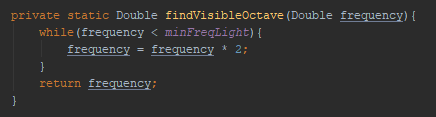
\includegraphics[]{visibleOctave}
\caption{Transformare frecvență}
\label{fig:visibleOctave}
\end{figure} 
Pentru a găsi lungimea de undă corespunzătoare în acest caz frecvența va fi cu aproximativ 40 de octave mai sus decât cea inițială, ceea ce este mult peste ce poate un om să audă. Cu frecvența corespunzătoare notei muzicale respective putem să calculăm lungimea de undă și să găsim un interval în care se potrivește pentru reprezentarea culorii.
\\
\par Algoritmul ales pentru a converti lungimile de undă în culori folosește modelul RGB\footnote{Modelul de culoare roșu-verde-albastru} și pentru fiecare interval de culoare (în total 6 culori) calculează valorile acestora folosind și o corecție gamma. Se poate vedea un e\-xem-plu din acest algoritm pentru culoarea roșie în figura \ref{fig:red}.
\begin{figure}[h]
\centering
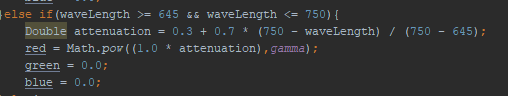
\includegraphics[]{red}
\caption{Exemplu calculare RGB}
\label{fig:red}
\end{figure} 
% a se adauga exemple cu culori
Datorită faptului că valorile RGB trebuie să fie cuprinse între 0 și 255, la sfârșit fiecare valoare se va înmulți cu 255 și se a returna un vector cu trei valori. Reprezentarea acestor culori se face cu ajutorul unui ImagevIew astfel se va folosi metoda \verb|setBackgrounColor()| unde se vor da ca parametrii cele trei valori calculate. Pentru că programul rulează pe mai multe fire de execuție, iar calcularea valorlor RGB se întâmplă pe un thread separat pentru a nu-l bloca pe cel principal, trebuie să avem în vedere faptul că nu putem să facem modificări pe UI atâta timp cât noi suntem pe un fir de execuție "muncitor" (adică care nu se ocupă de aspecte cum ar fi desenarea UI-ului sau răspunderea la interacțiunile utilizatorilor). Pentru a rezolva această problemă am utilizat metoda \verb|runOnUiThread()|. Primind ca parametru un nou \verb|Runnable|, metoda a determina executarea codului pe firul principal de execuție. Apelarea acestei metode este posibil numai în cazul în care suntem în clasa \verb|MainActivity|, fiind o metodă a obiectului \verb|Activity|.
\\
\par Fiecare notă muzicală dintr-o octavă va avea culori diferite ceea ce înseamnă că nu se va diferenția prin culori faptul că nota cântată a fost una adâncă sau înaltă, acest lucru putând fi diferențiat numai prin vibrațiile simțite. Datorită faptului că frecvența inițială se înmulțește până când rezultatul este o una la care ochiul uman ar percepe culorile, secvența culorilor dintr-o octavă nu va urmări în totalitate ordinea culorilor din spectrul vizibil. Asta înseamnă că prima notă din octavă, care ar trebui să aibă cea mai mică frecvență și cea mai mare lungime de undă, nu va avea culoarea roșie. Însă se poate observa diferența minimală de culori dintre notele unele note adiacente. De exemplu notele fa, fa$\sharp$ și sol au toate o tentă de culoare roșie. Exemplele de culori pentru fiecare notă pe care le-am obținut în urma implementării algoritmul se pot observa în figura \ref{fig:colors}.
\begin{figure}[h]
\centering
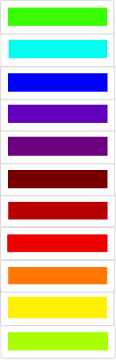
\includegraphics[scale = 1.1,angle = 90]{colors}
\caption{Culori octavă}
\label{fig:colors}
\end{figure} 
\end{document}